\chapter{RESULTADOS E DISCUSS�O}
\label{resultados}
Neste cap�tulo, ser� apresentado algumas imagens de terrenos gerados (Se��o \ref{terrenosgerados}) e tamb�m algum testes executados (\ref{testes}).


\section{Terrenos gerados}
\label{terrenosgerados}

A Figura \ref{fig:heightmap2} mostra a renderiza��o de uma cena apenas com a textura do mapa de altura aplicado em um quadrado.
\begin{figure}[H]
	\center{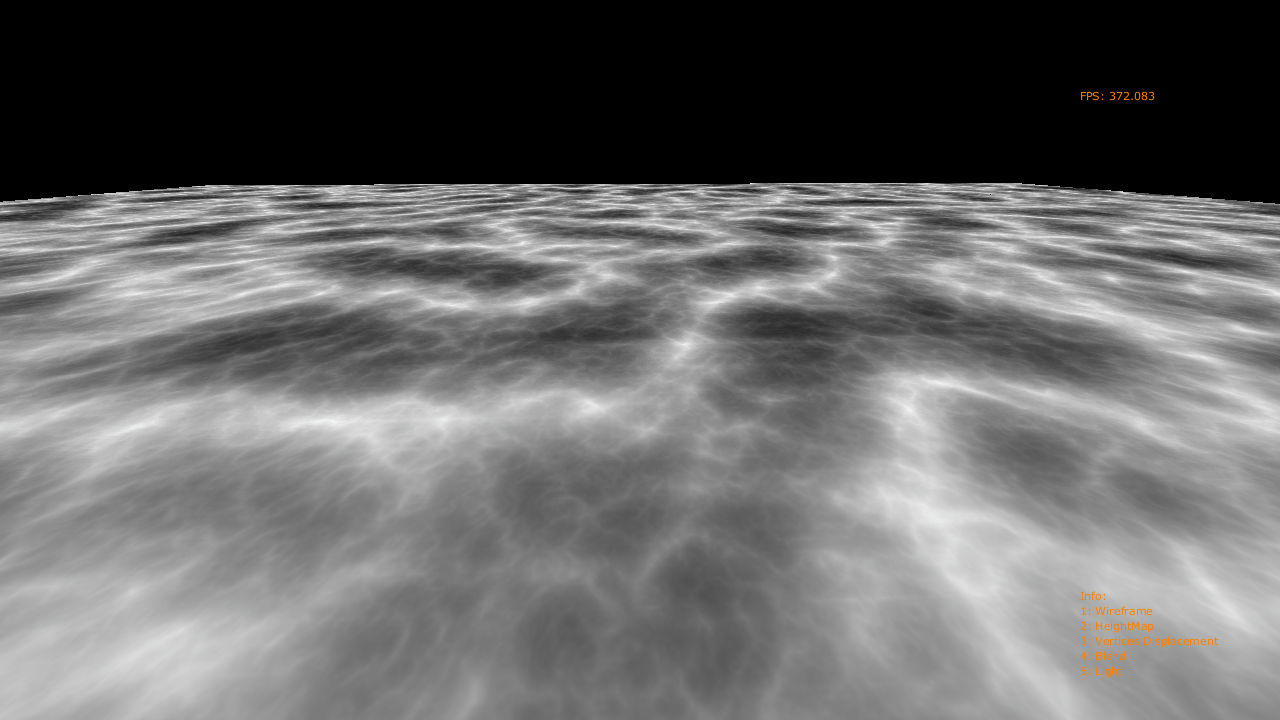
\includegraphics[width=0.5\linewidth]{img/caps/heightmap2.png}}
	\caption{\label{fig:heightmap2} Mapa de altura aplicado a um quadrado.}
\end{figure}


A Figura \ref{fig:deslocamento} mostra o mesmo mapa de altura, mas agora com o deslocamento dos v�rtices em no eixo \emph{z}.
\begin{figure}[H]
	\center{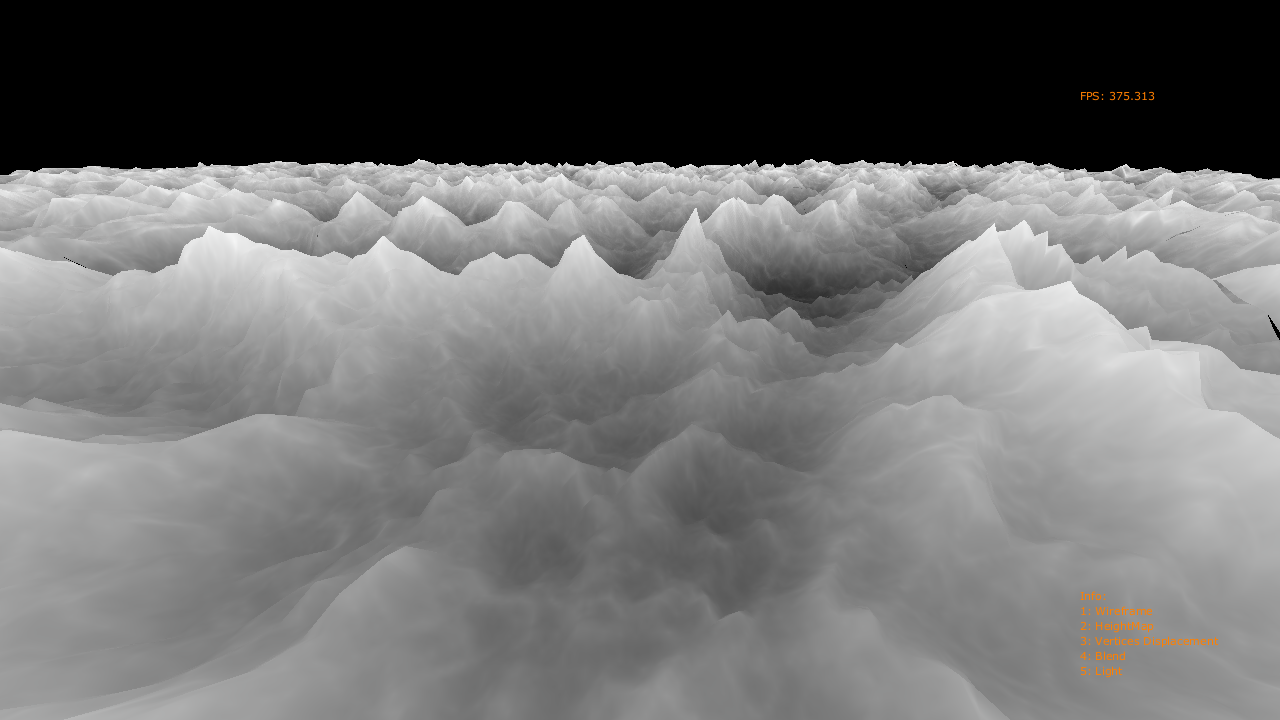
\includegraphics[width=0.5\linewidth]{img/caps/deslocamento.png}}
	\caption{\label{fig:deslocamento} Mapa de altura aplicado a um quadrado, deslocando a altura.}
\end{figure}

A Figura \ref{fig:blend} mostra agora a renderiza��o da malha com texturas para simular grama, pedras, neve, etc.
\begin{figure}[H]
	\center{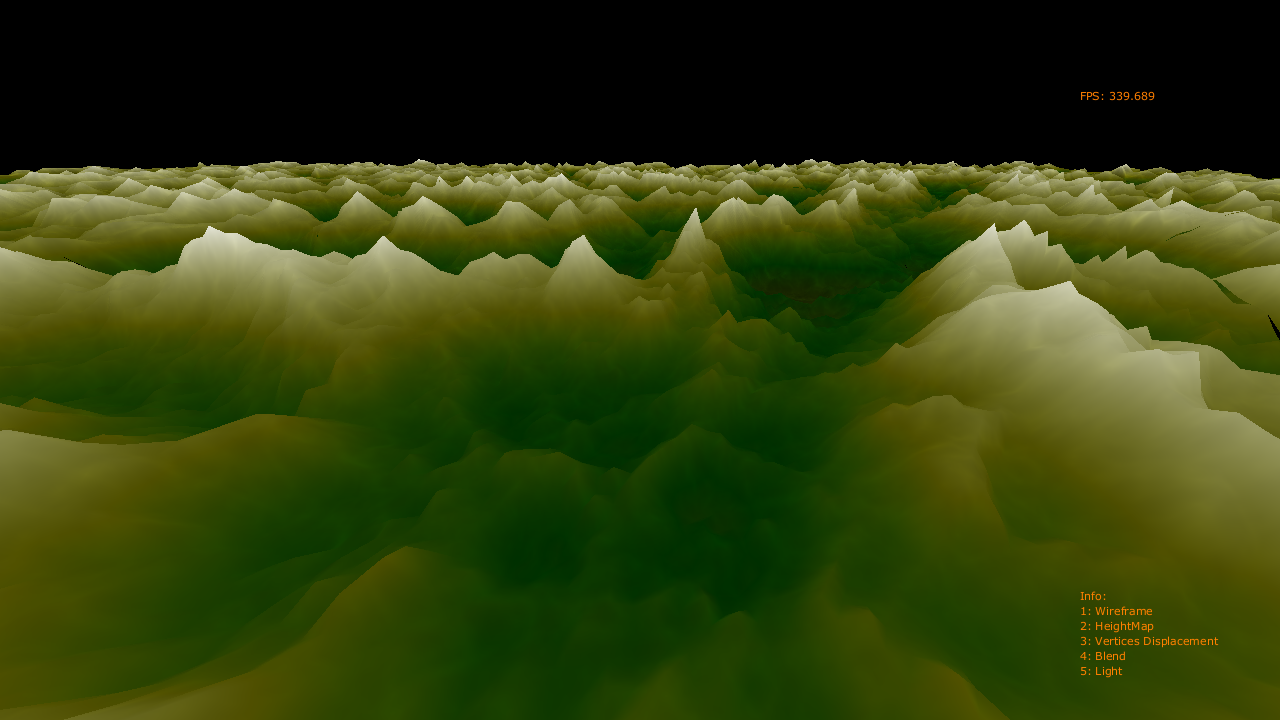
\includegraphics[width=0.5\linewidth]{img/caps/blend.png}}
	\caption{\label{fig:blend} Mapa de altura aplicado a um quadrado, deslocando a altura, e com texturas.}
\end{figure}

A Figura \ref{fig:luz} mostra o resultado final, agora com a aplica��o de ilumina��o.
\begin{figure}[H]
	\center{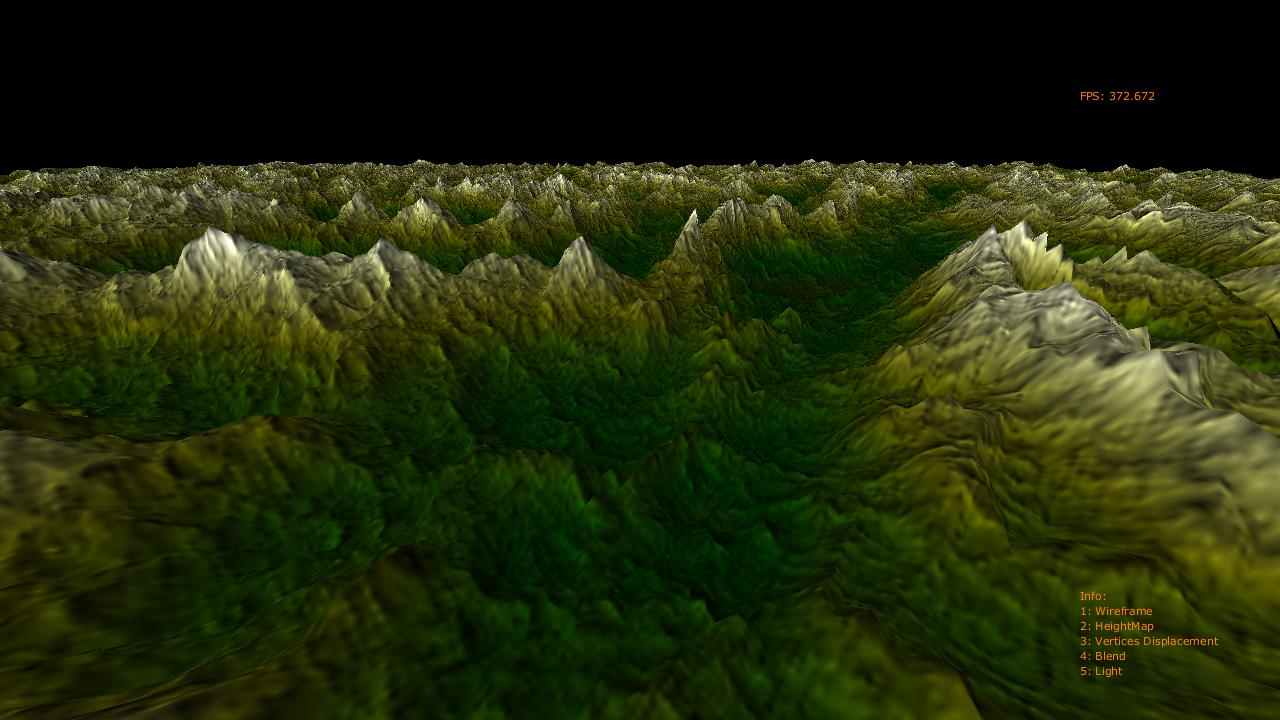
\includegraphics[width=0.5\linewidth]{img/caps/luz.png}}
	\caption{\label{fig:luz} Mapa de altura aplicado a um quadrado, deslocando a altura, com texturas, e ilumina��o.}
\end{figure}

Um v�deo demonstrando mostrando a navega��o pelo terreno pode ser visto em \cite{youtube}.


\section{Testes de Desempenho}
\label{testes}
Alguns testes foram feitos para avaliar a velocidade de gera��o dos terrenos com a altera��o de alguns par�metros, utilizando tanto a GPU quanto a CPU. Eles foram executados em um \emph{Core 2 Duo E7400}, com 2GB de mem�ria \emph{RAM} e placa de v�deo \emph{ATI Radeon HD 4850} com 512MB de mem�ria \emph{RAM}, e \emph{driver} vers�o 8.612. As tabelas com os tempos e as conclus�es dos testes s�o apresentadas a seguir.



\subsection{Tempos de Gera��o do Terreno}
\label{testeGeracao}
Neste teste foi medido o tempo m�dio gasto com a gera��o de terrenos tanto na \emph{GPU} quanto na \emph{CPU}. Os seguintes par�metros foram utilizados:

\begin{itemize}
\item \emph{Octaves}: Vari�vel (4, 8, 12, 16)
\item \emph{Lacunarity}: 2.5
\item Ganho: 0.5
\item \emph{Offset}: 1.0
\item Tamanho da textura: 512
\item N�mero de divis�es dos quadrados: 150
\item Tamanho dos quadrados: 5.0
\item Fator \emph{LOD}: 2
\end{itemize}



\begin{table}[H]
	\begin{center}
		\begin{tabular}{|c|c|c|}
			\hline
			\emph{Octaves} & GPU & CPU \\
			\hline
			4 & 28,7236 & 46,2948\\
			\hline
			8 & 28,7432 & 92,4299\\
			\hline
			16 & 28,7887 & 187,103\\
			\hline
			32 & 30,1095 & 370,841\\
			\hline
		\end{tabular}
		\caption{Tempo m�dio (em ms) de gera��o dos terrenos, com n�mero vari�vel de \emph{octaves}}
		\label{tabela:geracao}
	\end{center}
\end{table}


A Figura \ref{fig:geracao} apresenta os tempos anteriores.
\begin{figure}[H]
	\center{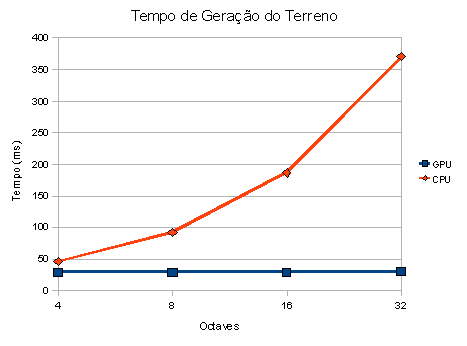
\includegraphics[width=0.4\linewidth]{img/tempoGeracao.png}}
	\caption{\label{fig:geracao} Gr�fico do tempo m�dio (em ms) de gera��o dos terrenos, com n�mero vari�vel de \emph{octaves}.}
\end{figure}


Como pode ser visto, o tempo de gera��o do terreno na \emph{GPU} permanece quase constante, enquanto a gera��o na \emph{CPU} tem um comportamento praticamente linear.


\subsection{\emph{Frames} por Segundo Durante Navega��o}
\label{testeFPS}
Neste teste foi medido o \emph{Frames por segundo} (\sigla{FPS}{Frames por segundo}) m�dio durante a navega��o pelo terreno gerado proceduralmente, por 30 segundos. Os seguintes par�metros foram utilizados:

\begin{itemize}
\item \emph{Octaves}: 16
\item \emph{Lacunarity}: 2.5
\item Ganho: 0.5
\item \emph{Offset}: 1.0
\item Tamanho da textura: 512
\item N�mero de divis�es dos quadrados: 150
\item Tamanho dos quadrados: 5.0
\item Fator \emph{LOD}: 2
\end{itemize}

A Tabela \ref{tabela:fps} mostra os tempos m�dios, m�nimos e a m�dia de \emph{FPS}. Al�m disso, h� o n�mero de \emph{frames} renderizados durante o percurso:

\begin{table}[H]
	\begin{center}
		\begin{tabular}{|c|c|c|c|c|}
			\hline
			 & Total de \emph{Frames} & \emph{FPS} M�nimo & \emph{FPS} M�ximo & \emph{FPS} M�dio \\
			\hline
			CPU & 9664 & 248 & 397 & 322.133\\
			\hline
			GPU & 11287 & 361 & 394 & 376.233\\
			\hline
		\end{tabular}
		\caption{Dados sobre a navega��o pelo mundo durante 30 segundos}
		\label{tabela:fps}
	\end{center}
\end{table}


A Figura \ref{fig:fps} apresenta os tempos anteriores:
\begin{figure}[H]
	\center{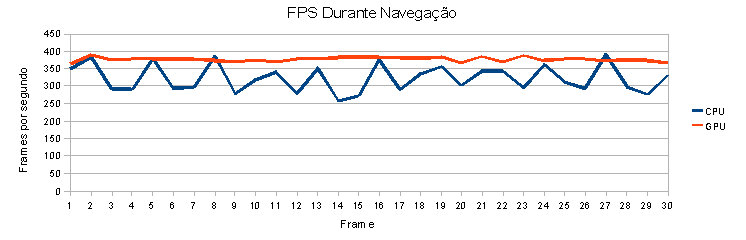
\includegraphics[width=0.9\linewidth]{img/tempoFPS.png}}
	\caption{\label{fig:fps} Gr�fico com o FPS na navega��o pelo mundo durante 30 segundos.}
\end{figure}


Como pode ser visto atrav�s do gr�fico, a navega��o pelo mundo, utilizando a gera��o dos terrenos na GPU, � muito mais fluida, sem quedas bruscas de \emph{FPS}, como nos \emph{frames} 3, 6, 9, 12, 14, 17, 20, 23, 26 e 29, gra�as �s centenas de unidades de processamento presentes na GPU.

Na gera��o pela CPU, tais quedas correspondem justamente aos momentos em que o sistema gera novos terrenos e podem significar um menor senso de imers�o do usu�rio no mundo virtual.

